%%%%%%%%%%%%%%%%%%%%%%%%%%%%%%%%%%%%
% Slide options
%%%%%%%%%%%%%%%%%%%%%%%%%%%%%%%%%%%%

% Option 1: Slides with solutions

\documentclass[slidestop,compress,mathserif]{beamer}
\newcommand{\soln}[1]{\textit{#1}}
\newcommand{\solnGr}[1]{#1}

\usepackage{tikz}
\usetikzlibrary{shapes, positioning}

% Option 2: Handouts without solutions

%\documentclass[11pt,containsverbatim,handout]{beamer}
%\usepackage{pgfpages}
%\pgfpagesuselayout{4 on 1}[letterpaper,landscape,border shrink=5mm]
%\newcommand{\soln}[1]{ }
%\newcommand{\solnGr}{ }

%%%%%%%%%%%%%%%%%%%%%%%%%%%%%%%%%%%%
% Style
%%%%%%%%%%%%%%%%%%%%%%%%%%%%%%%%%%%%

\def\chpii@path{../../Chp 2}
\input{../../lec_style.tex}


%%%%%%%%%%%%%%%%%%%%%%%%%%%%%%%%%%%%
% Preamble
%%%%%%%%%%%%%%%%%%%%%%%%%%%%%%%%%%%%

\title[Lecture 5]{MA 213: Lecture 5}
\subtitle{Module 1: Exploratory Data Analysis and Study Design}
\author{OpenIntro Statistics, 4th Edition}
\institute{$\:$ \\ {\footnotesize Based on slides developed by Mine \c{C}etinkaya-Rundel of OpenIntro. \\
The slides may be copied, edited, and/or shared via the \webLink{http://creativecommons.org/licenses/by-sa/3.0/us/}{CC BY-SA license.} \\
Some images may be included under fair use guidelines (educational purposes).\\
\\
Dolphin Case Study adapted from Nathan Tintle et al., ``Teaching Statistics with Active Investigations'', April 8, 2025, Instats.}}
\date{}

%%%%%%%%%%%%%%%%%%%%%%%%%%%%%%%%%%%%
% Begin document
%%%%%%%%%%%%%%%%%%%%%%%%%%%%%%%%%%%%

\begin{document}


%%%%%%%%%%%%%%%%%%%%%%%%%%%%%%%%%%%%
% Title page
%%%%%%%%%%%%%%%%%%%%%%%%%%%%%%%%%%%%

{
\addtocounter{framenumber}{-1} 
{\removepagenumbers 
\usebackgroundtemplate{\includegraphics[width=\paperwidth]{../../OpenIntro_Grid_4_3-01.jpg}}
\begin{frame}

\hfill \includegraphics[width=20mm]{../../oiLogo_highres}

\titlepage

\end{frame}
}
}

%%%%%%%%%%%%%%%%%%%%%%%%%%%%%%%%%%%%
% Sections
%%%%%%%%%%%%%%%%%%%%%%%%%%%%%%%%%%%%


%%%%%%%%%%%%%%%%%%%%%%%%%%%%%%%%%%%%
% Recap/Agenda 
%%%%%%%%%%%%%%%%%%%%%%%%%%%%%%%%%%%%
% TODO better formatting
\begin{frame}
    \frametitle{Module 1: Exploratory Data Analysis and Study Design}
    \begin{itemize}
        \item \hl{Previously: } Considering categorial data (Chapter 2.2)
        \item \hl{This time: } Two case studies
        \item \hl{Reading: } Chapter 3.1 for next time
        \item \hl{Deadlines/Announcements: }Homework 2 Due Monday
    \end{itemize}
    
\end{frame}

%%%%%%%%%%%%%%%%%%%%%%%%%%%%%%%%%%%%
% Learning objectives:
%%%%%%%%%%%%%%%%%%%%%%%%%%%%%%%%%%%%
\begin{frame}
    \frametitle{Learning Objectives}
    \begin{itemize}
        \item \textbf{M1, LO3: Use R for Data Management and Exploration:} Utilize R to load, pre-process, and explore data through visualization and summarization techniques.
        \item \textbf{M1, L05: Conduct Hypothesis Testing Using Simulation:} Set up null and alternative hypotheses to test for independence between variables, and use simulation techniques to evaluate data support for these hypotheses.
    \end{itemize}
\end{frame}


%%%%%%%%%%%%%%%%%%%%%%%%%%%%%%%%%%%%

\section{Case study: Dolphin communication}

%%%%%%%%%%%%%%%%%%%%%%%%%%%%%%%%%%%%

\begin{frame}
  \frametitle{Can dolphins communicate abstract ideas?}
    \begin{block}{Research Question}
        Can dolphins communicate more than simple emotions---can they send abstract messages to each other (e.g., ``Push the \textbf{left} button'')?
    \end{block}
    \vspace{0.5cm}
    \begin{itemize}
        \item Dolphins are known to communicate simple feelings.
        \item Dr. Jarvis Bastian designed an experiment to test for more complex communication.
    \end{itemize}
    \vspace{0.5cm}
    \begin{center}
      \begin{tikzpicture}[scale=1.5]
        \node at (-1,0) {
\includegraphics[width=2.5cm]{dolphin.pdf}};
        \node at (1,0) {\reflectbox{
\includegraphics[width=2.5cm]{dolphin.pdf}}};
        \node at (0,-0.5) {\Large\bfseries ?};
      \end{tikzpicture}
    \end{center}
\end{frame}

%%%%%%%%%%%%%%%%%%%%%%%%%%%%%%%%%%%%

\begin{frame}{Training Phase 1: Learning Button Signals}
    \begin{block}{Setup}
        \begin{itemize}
            \item Each dolphin has two buttons: left and right.
            \item Steady headlight: \textbf{Push right button.}
            \item Blinking headlight: \textbf{Push left button.}
            \item Correct response = fish reward!
        \end{itemize}
    \end{block}
    \bigskip
    \begin{center}
        \begin{tikzpicture}[scale=1.5]
            % Pool
            \draw[cyan, thick, fill=cyan!10] (-1.2,-0.5) rectangle (5.2,1.5);
            % Dolphins (unflipped left, flipped right)
            \node at (0,0.5) {
\includegraphics[width=1.8cm]{dolphin.pdf}};
            \node at (4,0.5) {\reflectbox{
\includegraphics[width=1.8cm]{dolphin.pdf}}};
            % Buttons for Doris (left dolphin)
            \draw[fill=red] (-0.6,1.25) circle (0.09);
            \draw[fill=green!60!black] (0.6,1.25) circle (0.09);
            % Buttons for Buzz (right dolphin)
            \draw[fill=red] (3.4,1.25) circle (0.09);
            \draw[fill=green!60!black] (4.6,1.25) circle (0.09);
            % Headlight (center, above pool)
            \node[star,star points=5,fill=yellow!80!orange!70,minimum size=0.32cm,draw] at (2,1.7) {};
            \node at (2,2.0) {\scriptsize Headlight (steady/blink)};
            % Labels
            \node at (0,-0.1) {Doris};
            \node at (4,-0.1) {Buzz};
        \end{tikzpicture}
    \end{center}
\end{frame}

%%%%%%%%%%%%%%%%%%%%%%%%%%%%%%%%%%%%

\begin{frame}{Training Phase 2: Buzz before Doris}
    \begin{itemize}
        \item Now, both must push correct buttons \textbf{in order:}
        \begin{itemize}
            \item Buzz goes first,
            \item then Doris.
        \end{itemize}
        \item Only correct order earns reward!
        \item Dolphins learn the new, more complex rule.
    \end{itemize}
    \vspace{0.3cm}
    \begin{center}
        \begin{tikzpicture}[scale=1.5]
            % Pool
            \draw[cyan, thick, fill=cyan!10] (-1.2,-0.5) rectangle (5.2,1.5);
            % Dolphins
            \node at (0,0.5) {
\includegraphics[width=1.8cm]{dolphin.pdf}};
            \node at (4,0.5) {\reflectbox{
\includegraphics[width=1.8cm]{dolphin.pdf}}};
            % Buttons for Doris
            \draw[fill=red] (-0.6,1.25) circle (0.09);
            \draw[fill=green!60!black] (0.6,1.25) circle (0.09);
            % Buttons for Buzz
            \draw[fill=red] (3.4,1.25) circle (0.09);
            \draw[fill=green!60!black] (4.6,1.25) circle (0.09);
            % Headlight
            \node[star,star points=5,fill=yellow!80!orange!70,minimum size=0.32cm,draw] at (2,1.7) {};
            \node at (2,2.0) {\scriptsize Headlight};
            % Arrow for order
             \draw[->,blue,very thick] (3.3,1.0) .. controls (2.7,1.5) and (1.2,1.5) .. (0.7,1.0);
            \node[blue] at (2,1.1) {\scriptsize Buzz first, then Doris};
            % Labels
            \node at (0,-0.1) {Doris};
            \node at (4,-0.1) {Buzz};
        \end{tikzpicture}
    \end{center}
\end{frame}

%%%%%%%%%%%%%%%%%%%%%%%%%%%%%%%%%%%%

\begin{frame}{Final Phase: The Curtain Test}
    \begin{itemize}
        \item A curtain is placed between the dolphins.
        \item Only Doris can see the headlight; Buzz cannot.
        \item Can Doris \textbf{tell} Buzz which button to push, using only sounds?
    \end{itemize}
    \vspace{0.25cm}
    \begin{center}
    \begin{tikzpicture}[scale=1.5]
      % Pool
      \draw[cyan, thick, fill=cyan!10] (-1.2,-0.5) rectangle (5.2,1.5);
      % Curtain
      \draw[very thick,gray] (2,1.5) -- (2,-0.5);
      \node[gray!80!black,rotate=90] at (1.8,0.3) {\small Curtain};
      % Dolphins (one flipped)
      \node at (0,0.5) {
\includegraphics[width=1.8cm]{dolphin.pdf}};
      \node at (4,0.5) {\reflectbox{
\includegraphics[width=1.8cm]{dolphin.pdf}}};
      % Headlight only on Doris's side
      \node[star,star points=5,fill=yellow!80!orange!70,minimum size=0.32cm,draw] at (0,1.7) {};
      \node at (0,2.0) {\scriptsize Headlight };
      % Whistling arrow
      \draw[->,blue,very thick] (0.7,1.0) .. controls (1.2,1.5) and (2.7,1.5) .. (3.3,1.0);
      \node[blue] at (2,1.1) {\footnotesize whistling};
      % Buttons
      \draw[fill=red] (-0.6,1.25) circle (0.09);
      \draw[fill=green!60!black] (0.6,1.25) circle (0.09);
      \draw[fill=red] (3.4,1.25) circle (0.09);
      \draw[fill=green!60!black] (4.6,1.25) circle (0.09);
      % Labels
      \node at (0,-0.1) {Doris};
      \node at (4,-0.1) {Buzz};
    \end{tikzpicture}
    \end{center}
\end{frame}

%%%%%%%%%%%%%%%%%%%%%%%%%%%%%%%%%%%%

\begin{frame}{Measurement}
    \begin{block}{Results}
        In one phase of the study:
        \begin{itemize}
            \item Buzz was given 16 trials to push the correct button,
            \item He chose correctly \textbf{15 out of 16 times.}
        \end{itemize}
    \end{block}
    \vspace{0.3cm}
    \begin{itemize}
        \item Proportion correct: \[\frac{15}{16} = 0.9375\; (93.75\%)\]
        \item What does this suggest? How likely is this by chance?
    \end{itemize}
    \vspace{0.5cm}
    \begin{center}
        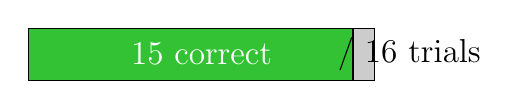
\begin{tikzpicture}[scale=1.1]
            \draw[fill=gray!40] (0,0) rectangle (4,0.6);
            \draw[fill=green!70!black!80] (0,0) rectangle (3.75,0.6);
            \node[white] at (2,0.3) {\large 15 correct};
            \node at (4.4,0.3) {\large / 16 trials};
        \end{tikzpicture}
    \end{center}
\end{frame}

%%%%%%%%%%%%%%%%%%%%%%%%%%%%%%%%%%%%

\begin{frame}{Think/Pair/Share}
    \begin{block}{2 mins Think, 5 mins Pair, 5 mins Share:}
        \begin{enumerate}
            \item Based on these data, do you think Buzz somehow knew which button to push?
            \item What are the two possible explanations for Buzz pushing the correct button most of the time?
            \item If you were trying to convince someone that Buzz \emph{wasn't just guessing}, how could you do it?
        \end{enumerate}
    \end{block}
    \vspace{0.6cm}
    \begin{center}
        \begin{tikzpicture}[scale=1.5]
            \node at (-1,0) {
\includegraphics[width=2.5cm]{dolphin.pdf}};
            \node at (1,0) {\reflectbox{
\includegraphics[width=2.5cm]{dolphin.pdf}}};
            \node at (0,-0.5) {\Large \textit{Let's talk about it!}};
        \end{tikzpicture}
    \end{center}
\end{frame}

%%%%%%%%%%%%%%%%%%%%%%%%%%%%%%%%%%%%
\begin{frame}{Possible Explanations}
    \begin{block}{Two possible explanations for Buzz's performance:}
        \begin{itemize}
            \item \textbf{Chance:} Buzz was just lucky, guessing correctly 15 out of 16 times.
            \item \textbf{Communication:} Doris communicated the correct button to push, and Buzz understood her signals.
        \end{itemize}
    \end{block}
\end{frame}

\begin{frame}{Convincing Someone Else}
    \begin{block}{Convincing someone that Buzz wasn't just guessing:}
        \begin{itemize}
            \item We can simulate the situation using coin flips.
            \item Each coin flip represents a trial where Buzz guesses.
            \item If we flip a coin 16 times, how many heads (correct guesses) do we expect?
            \item We can repeat this many times to see how often Buzz would get at least 15 heads by chance.
        \end{itemize}
    \end{block}
\end{frame}
%%%%%%%%%%%%%%%%%%%%%%%%%%%%%%%%%%%%

%%%%%%%%%%%%%%%%%%%%%%%%%%%%%%%%%%%%
\section{Applet: \href{https://www.isi-stats.com/isi2nd/ISIapplets2021.html}{Coin Flips}}
% https://www.isi-stats.com/isi2nd/ISIapplets2021.html
% One Proportion
%%%%%%%%%%%%%%%%%%%%%%%%%%%%%%%%%%%%

%%%%%%%%%%%%%%%%%%%%%%%%%%%%%%%%%%%%
\begin{frame}{Parallels between simulation and real study}
\begin{table}
    \renewcommand{\arraystretch}{1.4} % increases table row height for readability
    %\rowcolors{2}{white}{blue!4!white}
    \begin{tabular}{p{3.0cm} c p{6.0cm}}
        \rowcolor{blue!30!black!15} 
        \textbf{Simulation} & & \textbf{Real Study}\\
        \hline
        Coin flip         & = & guess by Buzz \\
        Heads             & = & correct guess \\
        Tails             & = & wrong guess \\
        Chance of heads   & = & $1/2$, probability of correct button when Buzz is just guessing \\
        One repetition    & = & one set of 16 simulated attempts by Buzz \\
    \end{tabular}
\end{table}
\end{frame}

%%%%%%%%%%%%%%%%%%%%%%%%%%%%%%%%%%%%

\begin{frame}{Simulation-Based Inference: Big Picture}
    \begin{itemize}
        \item \hl{Statistic: }Compute the statistic from the observed data.
        \item \hl{Simulate: } Identify a model that represents a chance explanation. Repeatedly simulate 
        values of the statistic that could have happened when the chance model is true and form a distribution. 
        \item \hl{Strength of evidence: }Consider whether the value of the observed statistic is unlikely to occur
    \end{itemize}
\end{frame}

%%%%%%%%%%%%%%%%%%%%%%%%%%%%%%%%%%%%

\section{Case study: Gender discrimination}

%%%%%%%%%%%%%%%%%%%%%%%%%%%%%%%%%%%%

\subsection{Study description and data}

%%%%%%%%%%%%%%%%%%%%%%%%%%%%%%%%%%%%

\begin{frame}
\frametitle{Gender discrimination}

\begin{itemize}

\item In 1972, as a part of a study on gender discrimination, 48 male bank supervisors were each given the same personnel file and asked to judge whether the person should be promoted to a branch manager job that was described as ``routine". 

\item The files were identical except that half of the supervisors had files showing the person was male while the other half had files showing the person was female.

\item It was randomly determined which supervisors got ``male" applications and which got ``female" applications.  

\item Of the 48 files reviewed, 35 were promoted. 

\item The study is testing whether females are unfairly discriminated against.  
\end{itemize}

\dq{Is this an observational study or an experiment?} \soln{\onslide<2->{Experiment}}

\ct{B.Rosen and T. Jerdee (1974), ``Influence of sex role stereotypes on personnel decisions", J.Applied Psychology, 59:9-14.}

\end{frame}


%%%%%%%%%%%%%%%%%%%%%%%%%%%%%%%%%%%%

\begin{frame}
\frametitle{Data}

\dq{At a first glance, does there appear to be a relatonship between promotion and gender?}

\begin{center}
\begin{tabular}{ll  cc c} 
  		&				& \multicolumn{2}{c}{\textit{Promotion}} \\
\cline{3-4}
							&			& Promoted	& Not Promoted 	& Total	\\
\cline{2-5}
\multirow{2}{*}{\textit{Gender	}}	&Male 		& 21	 	& 3		& 24 	\\
							&Female		& 14	 	& 10 	 	& 24 \\
\cline{2-5}
							&Total		& 35		& 13		& 48 \\
\end{tabular}
\end{center}

\pause

\textbf{\% of males promoted: $21 / 24 = 0.875$} \\
\textbf{\% of females promoted: $14 / 24 = 0.583$}

\end{frame}

%%%%%%%%%%%%%%%%%%%%%%%%%%%%%%%%%%%%

\begin{frame}
\frametitle{Practice}

\pq{We saw a difference of almost 30\% (29.2\% to be exact) between the proportion of male and female files that are promoted. Based on this information, which of the below is true?}

\begin{enumerate}[(a)]

\item If we were to repeat the experiment we will definitely see that more female files get promoted. This was a fluke.

\item Promotion is dependent on gender, males are more likely to be promoted, and hence there is gender discrimination against women in promotion decisions. \soln{\only<2>{\red{Maybe}}}

\item The difference in the proportions of promoted male and female files is due to chance, this is not evidence of gender discrimination against women in promotion decisions. \soln{\only<2>{\red{Maybe}}}

\item Women are less qualified than men, and this is why fewer females get promoted.

\end{enumerate}

\end{frame}

%%%%%%%%%%%%%%%%%%%%%%%%%%%%%%%%%%%%

\subsection{Competing claims}

%%%%%%%%%%%%%%%%%%%%%%%%%%%%%%%%%%%%%

\begin{frame}
\frametitle{Two competing claims}

\begin{enumerate}

\item ``There is nothing going on." \\
Promotion and gender are \hl{independent}, no gender discrimination, observed difference in proportions is simply due to chance. $\rightarrow$ \hl{Null hypothesis}

\pause

\item ``There is something going on." \\
Promotion and gender are \hl{dependent}, there is gender discrimination, observed difference in proportions is not due to chance. $\rightarrow$ \hl{Alternative hypothesis}

\end{enumerate}

\end{frame}

%%%%%%%%%%%%%%%%%%%%%%%%%%%%%%%%%%%%

\begin{frame}
\frametitle{A trial as a hypothesis test}

\twocol{0.5}{0.5}
{
\begin{itemize}

\item Hypothesis testing is very much like a court trial.

\item $H_0$: Defendant is innocent \\
$H_A$: Defendant is guilty

\item We then present the evidence - collect data.

\end{itemize}
}
{
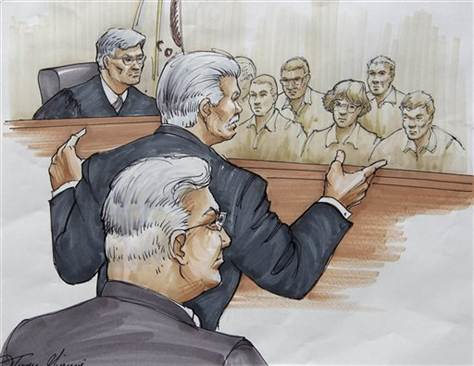
\includegraphics[width=\textwidth]{\chpii@path/2-3_gender_discrimination/figures/trial}
}

\begin{itemize}

\item Then we judge the evidence - ``Could these data plausibly have happened by chance if the null hypothesis were true?"
\begin{itemize}
\item If they were very unlikely to have occurred, then the evidence raises more than a reasonable doubt in our minds about the null hypothesis.
\end{itemize}

\item Ultimately we must make a decision. How unlikely is unlikely?

\end{itemize}

\ct{Image from \webURL{http://www.nwherald.com/_internal/cimg!0/oo1il4sf8zzaqbboq25oevvbg99wpot}.}

\end{frame}

%%%%%%%%%%%%%%%%%%%%%%%%%%%%%%%%%%%%%

\begin{frame}
\frametitle{A trial as a hypothesis test (cont.)}

\begin{itemize}

\item If the evidence is not strong enough to reject the assumption of innocence, the jury returns with a verdict of ``not guilty".
\begin{itemize}
\item The jury does not say that the defendant is innocent, just that there is not enough evidence to convict.
\item The defendant may, in fact, be innocent, but the jury has no way of being sure.
\end{itemize}

\item Said statistically, we fail to reject the null hypothesis.
\begin{itemize}
\item We never declare the null hypothesis to be true, because we simply do not know whether it's true or not.
\item Therefore we never ``accept the null hypothesis".
\end{itemize}

\end{itemize}

\end{frame}

%%%%%%%%%%%%%%%%%%%%%%%%%%%%%%%%%%%%%

\begin{frame}
\frametitle{A trial as a hypothesis test (cont.)}

\begin{itemize}

\item In a trial, the burden of proof is on the prosecution.

\item In a hypothesis test, the burden of proof is on the unusual claim.

\item The null hypothesis is the ordinary state of affairs (the status quo), so it's the alternative hypothesis that we consider unusual and for which we must gather evidence.

\end{itemize}

\end{frame}

%%%%%%%%%%%%%%%%%%%%%%%%%%%%%%%%%%%%%

\begin{frame}
\frametitle{Recap: hypothesis testing framework}

\begin{itemize}
\item We start with a \hl{null hypothesis ($H_0$)} that represents the status quo.
\item We also have an \hl{alternative hypothesis ($H_A$)} that represents our research question, i.e. what we're testing for.
\item We conduct a hypothesis test under the assumption that the null hypothesis is true, either via simulation (today) or theoretical methods (later in the course).
\item If the test results suggest that the data do not provide convincing evidence for the alternative hypothesis, we stick with the null hypothesis. If they do, then we reject the null hypothesis in favor of the alternative.
\end{itemize}

\end{frame}

%%%%%%%%%%%%%%%%%%%%%%%%%%%%%%%%%%%%

\subsection{Testing via simulation}

%%%%%%%%%%%%%%%%%%%%%%%%%%%%%%%%%%%%%

\begin{frame}
\frametitle{Simulating the experiment...}

... under the assumption of independence, i.e. leave things up to chance. \\

\vspace{0.5cm}

If results from the simulations based on the \hl{chance model} look like the data, then we can determine that the difference between the proportions of promoted files between males and females was simply \hl{due to chance} (promotion and gender are independent). \\

\vspace{0.5cm}

If the results from the simulations based on the chance model do not look like the data, then we can determine that the difference between the proportions of promoted files between males and females was not due to chance, but \hl{due to an actual effect of gender} (promotion and gender are dependent).

\end{frame}

%%%%%%%%%%%%%%%%%%%%%%%%%%%%%%%%%%%%

\begin{frame}
\frametitle{Application activity: simulating the experiment}

\app{
Use a deck of playing cards to simulate this experiment.

\begin{enumerate}
\item Let a face card represent \textit{not promoted} and a non-face card represent a \textit{promoted}. Consider aces as face cards.
\begin{itemize}
\item Set aside the jokers.
\item Take out 3 aces $\rightarrow$ there are exactly 13 face cards left in the deck (face cards: A, K, Q, J).
\item Take out a number card $\rightarrow$ there are exactly 35 number (non-face) cards left in the deck (number cards: 2-10).
\end{itemize}
\item Shuffle the cards and deal them intro two groups of size 24, representing males and females. 
\item Count and record how many files in each group are promoted (number cards).

\item Calculate the proportion of promoted files in each group and take the difference (male - female), and record this value.

\item Repeat steps 2 - 4 many times.

\end{enumerate}
}

\end{frame}

%%%%%%%%%%%%%%%%%%%%%%%%%%%%%%%%%%%%

\begin{frame}
\frametitle{Step 1}

\begin{center}
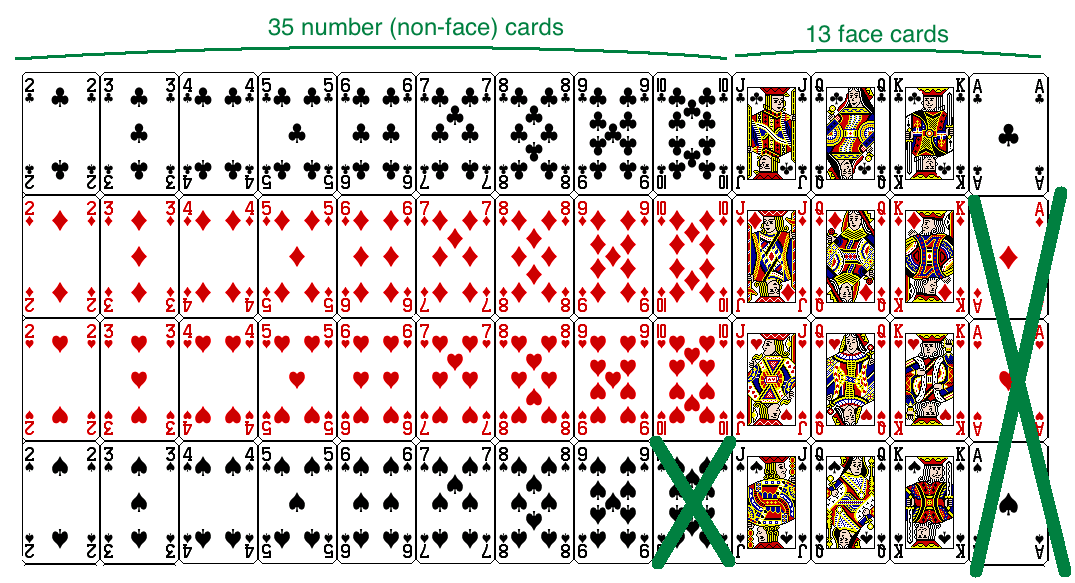
\includegraphics[width=\textwidth]{\chpii@path/2-3_gender_discrimination/figures/step1}
\end{center}

\end{frame}


%%%%%%%%%%%%%%%%%%%%%%%%%%%%%%%%%%%%

\begin{frame}
\frametitle{Step 2 - 4}

\begin{center}
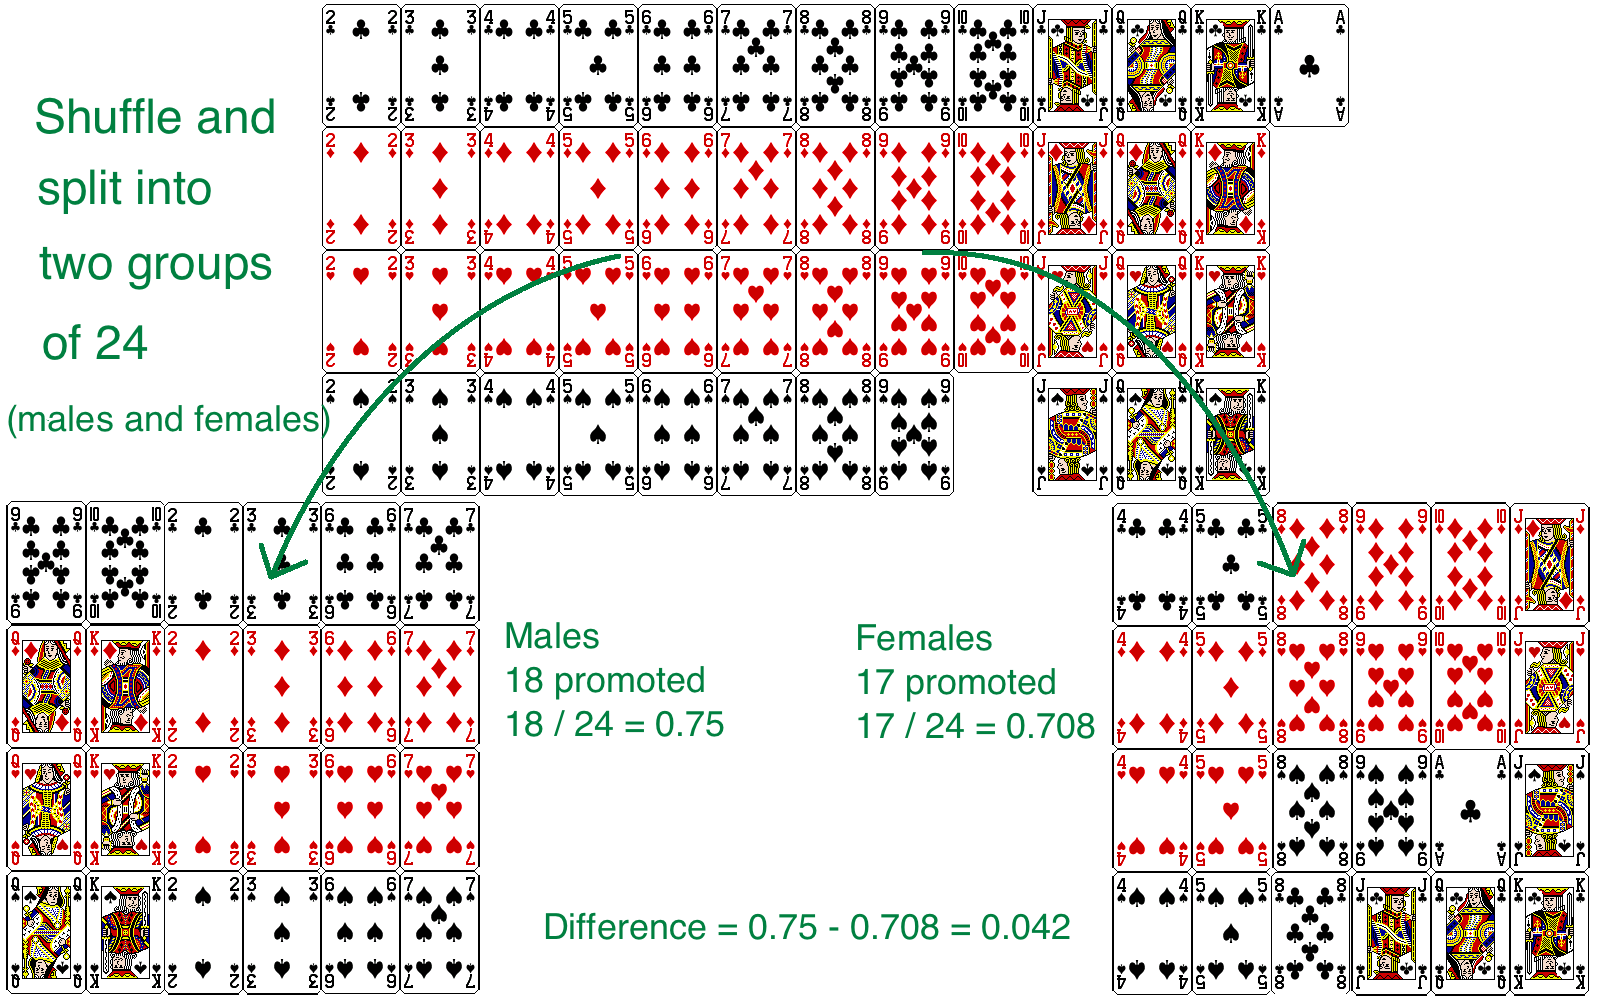
\includegraphics[width=\textwidth]{\chpii@path/2-3_gender_discrimination/figures/step2}
\end{center}

\end{frame}


%%%%%%%%%%%%%%%%%%%%%%%%%%%%%%%%%%%%

\subsection{Checking for independence}

%%%%%%%%%%%%%%%%%%%%%%%%%%%%%%%%%%%%

\begin{frame}
\frametitle{Practice}

\pq{Do the results of the simulation you just ran provide convincing evidence of gender discrimination against women, i.e. dependence between gender and promotion decisions?}

\begin{enumerate}[(a)]
\item No, the data do not provide convincing evidence for the alternative hypothesis, therefore we can't reject the null hypothesis of independence between gender and promotion decisions. The observed difference between the two proportions was due to chance.
\solnMult{Yes, the data provide convincing evidence for the alternative hypothesis of gender discrimination against women in promotion decisions. The observed difference between the two proportions was due to a real effect of gender.}
\end{enumerate}

\end{frame}

%%%%%%%%%%%%%%%%%%%%%%%%%%%%%%%%%%%%

\begin{frame}
\frametitle{Simulations using software}

These simulations are tedious and slow to run using the method described earlier. In reality, we use software to generate the simulations. The dot plot below shows the distribution of simulated differences in promotion rates based on 100 simulations.

\begin{center}
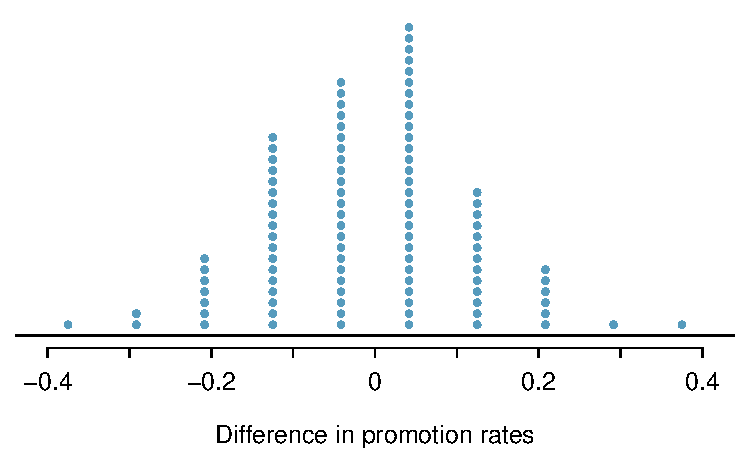
\includegraphics[width=0.8\textwidth]{\chpii@path/2-3_gender_discrimination/figures/discRandDotPlot/discRandDotPlot}
\end{center}

\end{frame}

%%%%%%%%%%%%%%%%%%%%%%%%%%%%%%%%%%%%%

%%%%%%%%%%%%%%%%%%%%%%%%%%%%%%%%%%%%
% End document
%%%%%%%%%%%%%%%%%%%%%%%%%%%%%%%%%%%%

\end{document}